\section{Results}
\newcommand{\FinalWarningScenarios}{81}
\newcommand{\FinalTrueWarnings}{10}
\newcommand{\FinalConservativeWarnings}{32}
\newcommand{\FinalSimultaneousWarnings}{39}
\newcommand{\FinalRobustWarnings}{4}
\newcommand{\FinalMSevenMisses}{20}
\newcommand{\FinalRhoJump}{406.0978}
\newcommand{\FinalGTwo}{4.21649}
\newcommand{\FinalGInf}{5.16703}
\newcommand{\FinalGradientValid}{0}
\newcommand{\FinalFallback}{1}

% Auto-generated from immutable Phase 2M-FOLLOWUP logs; do not edit numerically.
\newcommand{\FollowupScenarioCount}{81}
\newcommand{\FollowupTrueWarningCount}{10}
\newcommand{\FollowupConservativeWarningCount}{32}
\newcommand{\FollowupSimultaneousWarningCount}{39}
\newcommand{\FollowupMissedWarningCount}{0}
\newcommand{\FollowupRobustTrueWarningCount}{4}
\newcommand{\FollowupMaxGTwo}{4.21649}
\newcommand{\FollowupMaxGInf}{5.16703}


\subsection{Model-Based Feasibility and Allocation Evidence}
The broad M1 grid shows a dual-brake increase in signed reserve at 192 of 288 matched points, while both formulations are feasible at the same 270 points. To resolve what happens at the boundary, we held speed at 15~m/s and downgrade at 10\%, and varied initial brake temperature from 365 to 461~K and initial bumper gap from 15 to 90~m. Figure~\ref{fig:feasibility-frontier} shows the exact initial hard-command classification at 1,275 states: 1,071 friction-only feasible, 1,114 dual-brake feasible, and 43 feasible only with dual braking. At 413~K and 24~m, friction-only reserve is $-1.466$ whereas dual-brake reserve is $0.027$; the active friction and auxiliary upper bounds are respectively thermal and realized-force limits. This is a conditional one-step feasible-domain expansion, not a guarantee that every subsequent state remains feasible.

\begin{figure*}[t]
\centering
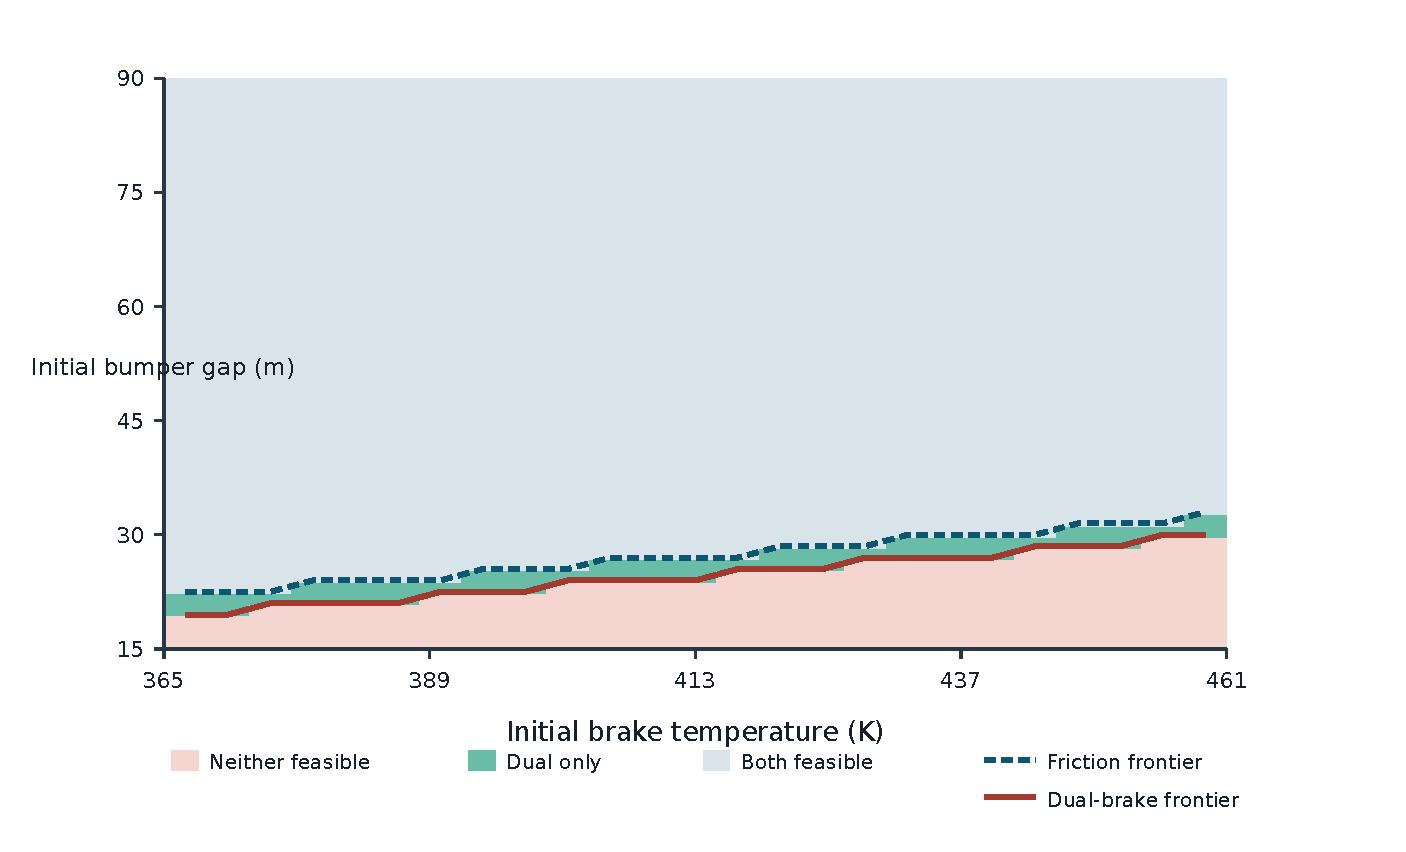
\includegraphics[width=.85\textwidth]{../generated/submission_revision/figures/feasibility_frontier.pdf}
\caption{Initial-command feasibility frontier at 15~m/s on a 10\% downgrade. Color classifies the declared two-command hard set at each initial temperature and bumper gap; dashed and solid lines mark the friction-only and dual-brake zero-reserve boundaries within the sampled domain. The green band is feasible only with auxiliary braking.}
\label{fig:feasibility-frontier}
\end{figure*}

All four M2 allocation strategies experience a negative minimum $\rho$ (Table~\ref{tab:phase2m-controller}); hence no strategy is described as universally safe. Allocation materially changes friction/auxiliary energy, tracking error, and peak temperature, but those matched model outcomes do not identify a learning advantage. M3 further records earlier certificate loss as the specified initial brake temperature approaches $T_{\rm crit}$; exact loss times and first critical components appear in Table~\ref{tab:final-model-evidence}.

A same-domain ablation retains the plant, hard rows, nominal dual-brake controller, disturbances, communication, and initial state while removing predictive/upstream triggering from the supervisor. In three 100-step, three-truck pairs, both versions have zero hard-certificate losses in ordinary and hot descents; both have six loss samples in the leader-braking case. Minimum reserves are identical within each pair (0.059, 0.023, and $-2.076$). Anticipatory mode is activated for 156, 300, and 294 truck-samples only in the proposed version, but this design does not show a closed-loop certificate-loss reduction. The full matched rows and comparison code are supplied with the source.

\begin{table*}[!t]
\centering\scriptsize
\caption{Selected model-based evidence from the Phase 2M analysis.}
\label{tab:final-model-evidence}
\begin{tabular}{llll}
\toprule
Study & Quantity & Result & Interpretation \\
\midrule
M1 & Dual/friction feasible points & 270/288; 270/288 & No feasible-count increase \\
M1 & Positive dual-reserve gain & 192/288 & Margin improvement only \\
M3 & Certificate loss at $T_0=413.7$ K & 16.4 s & collision\_demand \\
M3 & Certificate loss at $T_0=453.7$ K & 11 s & collision\_demand \\
M3 & Certificate loss at $T_0=461.7$ K & 10 s & collision\_demand \\
\bottomrule
\end{tabular}
\end{table*}

\begin{table*}[!t]
\centering
\scriptsize
\caption{Matched long-descent deterministic controller comparison.}
\label{tab:phase2m-controller}
\begin{tabular}{lrrrrr}
\hline
Method & Peak T (K) & Min. rho & Friction energy (MJ) & Auxiliary energy (MJ) & Speed root-mean-square error (m/s) \\
\hline
fixed\_auxiliary\_first & 458.81 & -28.532 & 12.265 & 25.978 & 2.8775 \\
fixed\_friction\_first & 458.8 & -10.141 & 13.233 & 24.796 & 2.3195 \\
friction\_only & 364.36 & -364.1 & 1.1293 & 0 & 15.938 \\
qp\_dual\_brake & 458.83 & -17.98 & 12.812 & 25.258 & 2.5585 \\
\hline
\end{tabular}
\end{table*}


\subsection{Predictive, Robustness, Communication, and Low-Speed Evidence}
The M4 case has neither a predictive crossing nor an observed instantaneous boundary, so it is inconclusive. M5 verifies the minimum-over-prefix horizon relation for every stored record; longer horizons can decrease the numerical predictive value, as Table~\ref{tab:phase2m-predictive} shows.

\begin{table*}[!t]
\centering
\scriptsize
\caption{Predictive-monitor and horizon metrics.}
\label{tab:phase2m-predictive}
\begin{tabular}{lrrrrrl}
\hline
Case & Trigger (s) & Boundary (s) & Warning (s) & Vehicle & Step & Component/status \\
\hline
M4 & -- & -- & -- & 1 & 3 & friction\_interval \\
M5 H=1 & -- & -- & -- & -- & -- & prefix monotonic=True \\
M5 H=3 & -- & -- & -- & -- & -- & prefix monotonic=True \\
M5 H=5 & 0 & -- & -- & -- & -- & prefix monotonic=True \\
M5 H=10 & 0 & -- & -- & -- & -- & prefix monotonic=True \\
\hline
\end{tabular}
\end{table*}


The targeted follow-up contains \FollowupScenarioCount{} boundary-approach scenarios: \FollowupTrueWarningCount{} isolated early warnings, \FollowupConservativeWarningCount{} warnings without a unique later boundary, and \FollowupSimultaneousWarningCount{} simultaneous crossings. Only \FollowupRobustTrueWarningCount{} early warnings satisfy the strict adjacent-grid and finite-margin rule. Figure~\ref{fig:predictive-examples} contrasts an isolated warning with a nonisolated case. Across 32,849 stored numerically positive predictive vehicle-samples, contemporaneous $\rho_i$ was never negative (minimum 0); this checks implementation consistency but not the sound-enclosure premise of Proposition~2. The tube regression checks 5,000 sampled states, not all future reachable states. A negative predictive value is an inconclusive warning, not proof of future infeasibility.

\begin{figure*}[t]
\centering
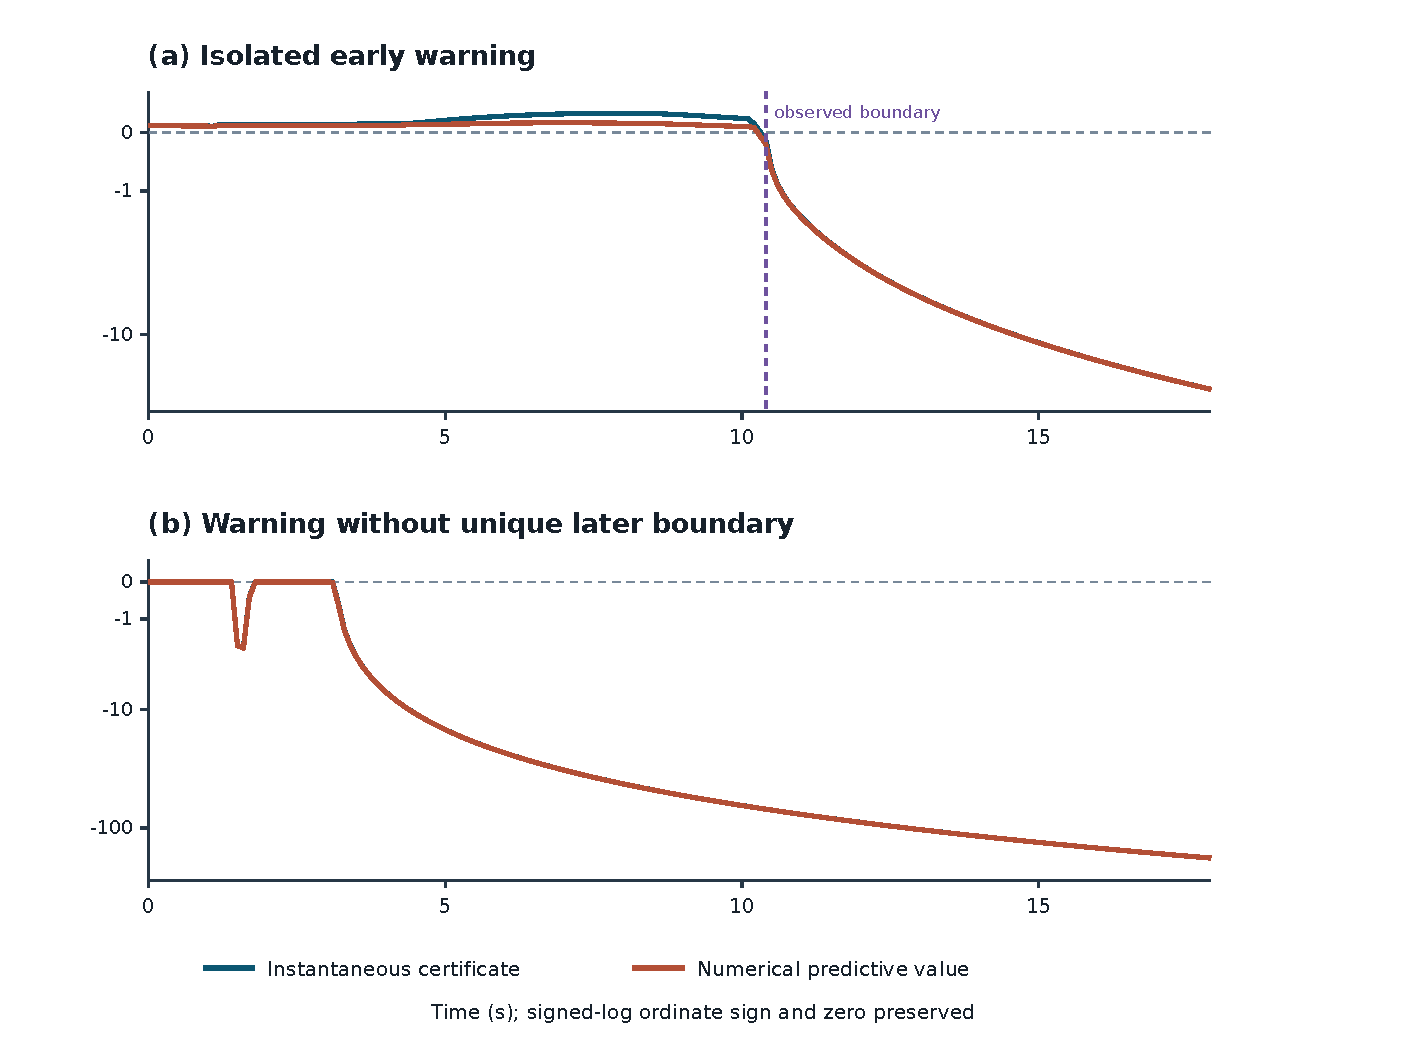
\includegraphics[width=.8\textwidth]{../generated/submission_revision/figures/predictive_examples.pdf}
\caption{Follower-1 instantaneous reserve and numerical predictive value in one isolated early-warning case (top) and one warning without a unique later boundary (bottom). The signed-log vertical mapping preserves the zero crossing while displaying the large negative tails; curves are model-based traces, not verified robust reachable-set bounds.}
\label{fig:predictive-examples}
\end{figure*}

M6 does not support a universal robustness claim. The deterministic endpoint set includes a certificate loss, and three of the 20 joint design-sensitivity samples lose the certificate. The joint set is not a physical probability distribution, so its loss frequency is not a reliability estimate; complete rows remain in the reproducibility package.

A separate 300-point stratified design varies the provenance-bounded mass, friction lag, cooling, and friction-force limit, plus auxiliary-capacity scale and digitization-bound fade-temperature offset around the 413-K/24-m boundary state. It yields 133 nonnegative initial reserves, with minimum $-1.505$ and maximum 0.059; collision demand limits 172 points and the auxiliary interval 128. This exposes sensitivity of boundary membership and normalized attribution, rather than a failure probability. Thermal capacity and auxiliary lag are held fixed because their declared intervals have zero width.

M7 and new fixed-delay runs quantify the cost of stale fleet awareness. At the head truck, mean absolute deviation from the centralized oracle grows from $3.1\times10^{-6}$ at zero delay to 0.027, 0.055, and 0.078 at 100, 200, and 300~ms. Under the 100-ms sample/consume schedule, nominal 50 and 100~ms configurations yield the same effective age and measured outcome. Head-truck critical-vehicle agreement drops from 1.00 at zero delay to 0.62, 0.64, and 0.62, respectively. The corresponding head missed/false trigger counts are 9/8, 7/10, and 6/11; therefore these counts are not monotone with delay, even though mean reserve error rises. Bounded-delay and stale-message cases reach a 1.118 mean head gap and 112 false triggers each. Figure~\ref{fig:communication} shows the deviation; the full channel metrics are archived. Vehicle-level agreement over all followers is lower even at zero delay because a non-head truck only aggregates its own upstream subchain.

\begin{figure*}[t]
\centering
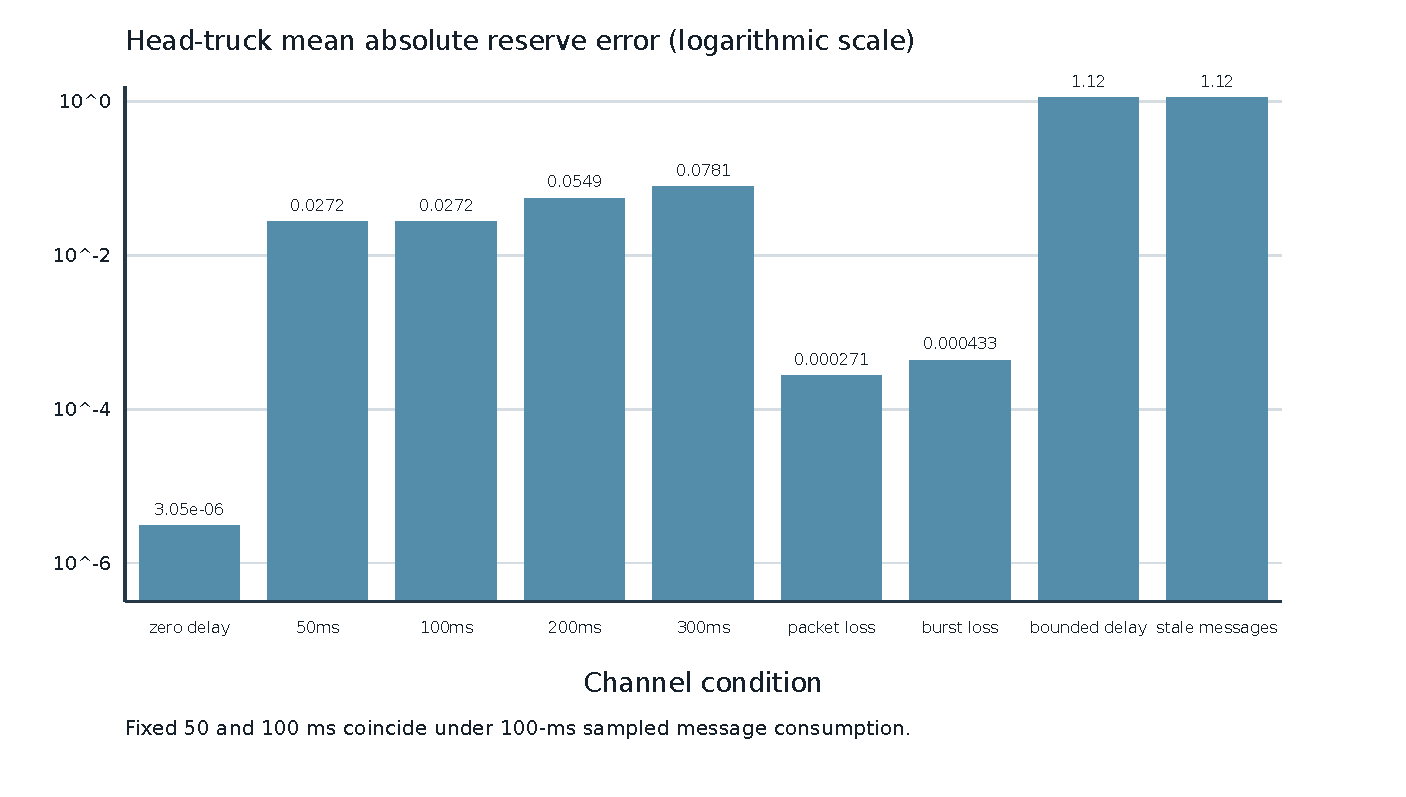
\includegraphics[width=.8\textwidth]{../generated/submission_revision/figures/communication_age.pdf}
\caption{Head-truck mean absolute deviation between the age-aware recursive reserve and instantaneous centralized oracle across fixed-delay and loss/staleness cases (logarithmic vertical scale). Each case contains 120 head-truck samples; the 50- and 100-ms delay cases coincide under 100-ms sampled consumption.}
\label{fig:communication}
\end{figure*}

M8 finds finite row evaluations but a hot-brake reserve jump across $v_\epsilon$: the ZOH and high-order barrier branches are different sufficient conditions, and their normalized reserves need not match. Because a smooth interpolation of sufficient conditions would not preserve the exact feasibility statement, we retain the hard switch and do not infer a physical feasibility discontinuity from its magnitude. The supervisor uses the actually active branch and reverifies every changed command. M9 does not satisfy the pre-registered numerical string-stability criterion in the tested grade-transition cases; string stability is an orthogonal performance property, not a theorem established here.

M10 measures computation only on the recorded Windows/Python test platform. The worst tested 99th-percentile controller time (P99) is below the 100-ms sampling period; component-wise measurements remain in the source package. This is neither target-hardware certification nor a real-time guarantee.

\subsection{Formal Learning and Conditional Differentiation}
Regular-case tests validate the local KKT derivative, but the calibrated paired-learning regime activates nonregular QP sets on every tested sample: the gradient-valid fraction is \FinalGradientValid{} and the fallback fraction \FinalFallback{}. DiffQP and matched StopGradient consequently have identical recorded returns and intervention outcomes in this campaign, with no evidence of a learning advantage. The forward safety projection remains unchanged. Detailed ten-seed protocol, paired outcomes, and gradient diagnostics are provided in the reproducibility package rather than promoted as a main feasibility result.

\subsection{Adapted External-Baseline Comparison}
The six deterministic matched heavy-duty transfer pairs have zero geometric collisions under both methods. The proposed method has lower peak brake temperature in each pair (362.43--461.71~K versus 479.24--658.92~K for the adapted Zhou \emph{et al.} controller) and no fade-envelope violation, while the transferred controller records 1,139 violations in total. These observations isolate a physical constraint class omitted by the scalar-acceleration source policy under the fixed adapter; they do not rank the native algorithms. Full per-case results and adapter code accompany the source package.

The post-hoc numerical evaluation of $\rho^{H,\mathrm{cert}}$ is negative for the adapted baseline in all six cases. The proposed method has negative predictive-monitor values in four cases and nonnegative values in two, so neither unconditional feasibility nor universal predictive superiority follows. Rather, the common feasibility monitor exposes collision--thermal conflicts that are not represented explicitly by the transferred collision-centric controller.

Lower speed root-mean-square error (RMSE), spacing RMSE, and jerk RMS are observed for the proposed method in all six matched pairs. Its traces use more auxiliary-braking energy in five cases and less friction-braking energy in all six, showing a systematic shift from friction toward auxiliary braking under the proposed allocator. These are observed deterministic matched outcomes, not general learning or energy-efficiency claims. The transferred baseline is computationally cheaper on the reported platform: its P99 runtime is 0.232--0.328~ms versus 1.037--1.522~ms. The proposed stack additionally evaluates thermal/fade hard rows, instantaneous feasibility, a predictive interval tube, a distributed bottleneck, and supervisor/reverification logic; the measured disadvantage is nevertheless retained and is not target-hardware real-time certification.

This comparison is adapter-sensitive because the source method outputs scalar acceleration while the heavy-duty plant requires friction/auxiliary commands. Observation mapping, the absence of heavy-duty retraining, and independently prespecified choices for unreported source details also affect the transfer. It is therefore a matched domain-transfer stress test, not a complete ranking of the algorithms in their native domains.

\section{Discussion and Limitations}
The primary contribution is feasibility certification and physical conflict attribution. The geometry makes the source of a feasibility loss inspectable: raising temperature contracts the friction interval; auxiliary braking may restore command authority, but only up to its own gear, speed, power, and lag bounds. The targeted frontier demonstrates a nonempty dual-only band under specified initial conditions, whereas the matched closed-loop ablation shows that predictive triggering need not reduce certificate losses in every tested disturbance. A certificate can therefore distinguish \emph{available authority} from \emph{realized supervisory benefit}. Its sign is invariant to positive normalizer changes, but limiting-component attribution is normalized: across the 288 M1 states, varying one of $s_f,s_a,s_M$ by 0.5 or 2 preserves every sign while component agreement ranges from 0.896 to 1.000. Trigger-time sensitivity was not measured and is not inferred from those snapshots.

Communication freshness controls the fidelity of fleet-level awareness. The head's zero-delay recursive minimum agrees with the centralized oracle, while delay, loss, and stale replacement alter both the value and its attribution. The framework can filter commands from different nominal controllers. Its theoretical finite-horizon guarantee requires sound uncertainty and reserve enclosures and final-action reverification; the present floating-point predictor lacks a verified enclosure proof. The low-speed switch remains discontinuous as a numerical certificate because its two sufficient conditions differ; no unsafe interpolation was introduced.

The plant is a literature-calibrated composite rather than an identified truck, and the lumped thermal model omits wheel-end imbalance and spatial gradients. There is no field or hardware-in-the-loop validation, analytical string-stability result, or universal closed-loop feasibility claim. Learning differentiation is secondary: persistent active-set degeneracy disables its QP-mediated backward path in the formal campaign. The external comparison is adapter-sensitive, and computation times apply only to the measured platform. These boundaries motivate identified thermal models and communication-aware validation in future work.
